\subsection*{An Algorithm in Linear Space}

The space complexity~(the memory required) of above algorithm~(DP-optimal-alignment) is $\Theta(mn)$,
as it maintains two matrices of size $(m+1)\cdot(n+1)$.  Can we do better?
First, if we only need the edit distance~(i.e., no need to reconstruct the optimal alignment), then linear space
is enough. This is because, the calculation of $F(i,j)$ only relies on two numbers in the previous row and
the one number in the current row. There is absolutely no need to restore the rows before the previous row.
Hence, we can modify that algorithm, by simply using two vectors and alternating them as previous and current rows.
The pseudo-code is given below. It runs in $\Theta(mn)$ time and in $\Theta(m+n)$ space.

\begin{algorithmblock}[0.8\textwidth]
	\aaA {8}{Algorithm DP-edit-distance~($X[1\cdots m]$, $Y[1\cdots n]$)}\xxx
	\aab {$F_1[j] = j$, for any $0 \le j \le n$}\xxx
	\aaB {5}{for $i = 1 \to m$}\xxx
	\aac {$F_2[0] = i$;}\xxx
	\aaC {2}{for $j = 1 \to n$}\xxx
	\aad {$F_2[j] = \min\{F_1[j-1] + \delta(X[i] \neq Y[j]), F_1[j] + 1, F_2[j-1] + 1\}$;}\xxx
	\aac {$F_1 = F_2$;}\xxx
	\aab {return: $F_1[n]$;}\xxx
\end{algorithmblock}

Note that, prior to the algorithm returns $F_1[n]$, 
$F_1[j]$ stores the length of the shortest path from $(0,0)$ to $(m, j)$ for
every $j = 0, 1, \cdots, n$. This inherits the definition of $F(i,j)$ in the DP-optimal-alignment,
which stores $d(X[1\cdots i], Y[1\cdots j])$, i.e., the length of the shortest path from $(0,0)$ to $(i,j)$.

\begin{figure}[b!]
\centering{

\tikzset{every picture/.style={line width=0.75pt}} %set default line width to 0.75pt        

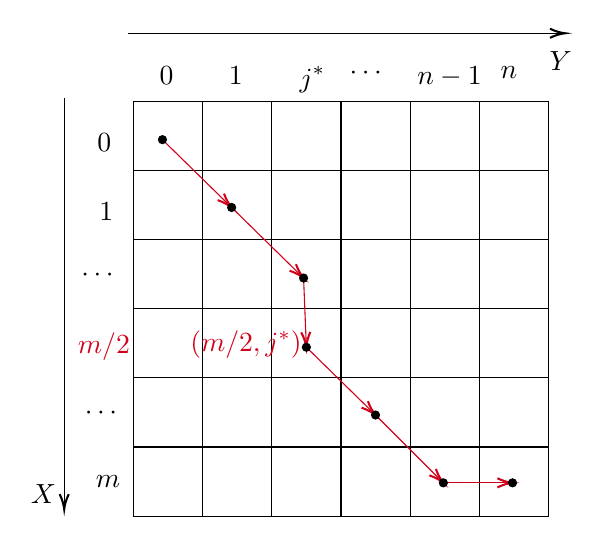
\begin{tikzpicture}[x=0.5pt,y=0.5pt,yscale=-1,xscale=1]
%uncomment if require: \path (0,424); %set diagram left start at 0, and has height of 424

%Shape: Grid [id:dp24675112085229023] 
\draw  [draw opacity=0] (87,90) -- (387,90) -- (387,390) -- (87,390) -- cycle ; \draw   (137,90) -- (137,390)(187,90) -- (187,390)(237,90) -- (237,390)(287,90) -- (287,390)(337,90) -- (337,390) ; \draw   (87,140) -- (387,140)(87,190) -- (387,190)(87,240) -- (387,240)(87,290) -- (387,290)(87,340) -- (387,340) ; \draw   (87,90) -- (387,90) -- (387,390) -- (87,390) -- cycle ;
%Straight Lines [id:da19565394910393163] 
\draw    (37,88) -- (37,383) ;
\draw [shift={(37,385)}, rotate = 270] [color={rgb, 255:red, 0; green, 0; blue, 0 }  ][line width=0.75]    (10.93,-3.29) .. controls (6.95,-1.4) and (3.31,-0.3) .. (0,0) .. controls (3.31,0.3) and (6.95,1.4) .. (10.93,3.29)   ;
%Straight Lines [id:da01702598838428071] 
\draw    (83,41) -- (397,41) ;
\draw [shift={(399,41)}, rotate = 180] [color={rgb, 255:red, 0; green, 0; blue, 0 }  ][line width=0.75]    (10.93,-3.29) .. controls (6.95,-1.4) and (3.31,-0.3) .. (0,0) .. controls (3.31,0.3) and (6.95,1.4) .. (10.93,3.29)   ;
%Straight Lines [id:da2874309790229619] 
\draw [color={rgb, 255:red, 208; green, 2; blue, 27 }  ,draw opacity=1 ]   (108,117.9) -- (156.57,165.5) ;
\draw [shift={(158,166.9)}, rotate = 224.42] [color={rgb, 255:red, 208; green, 2; blue, 27 }  ,draw opacity=1 ][line width=0.75]    (10.93,-3.29) .. controls (6.95,-1.4) and (3.31,-0.3) .. (0,0) .. controls (3.31,0.3) and (6.95,1.4) .. (10.93,3.29)   ;
%Straight Lines [id:da632617045829971] 
\draw [color={rgb, 255:red, 208; green, 2; blue, 27 }  ,draw opacity=1 ]   (262,316.9) -- (309.59,364.48) ;
\draw [shift={(311,365.9)}, rotate = 225] [color={rgb, 255:red, 208; green, 2; blue, 27 }  ,draw opacity=1 ][line width=0.75]    (10.93,-3.29) .. controls (6.95,-1.4) and (3.31,-0.3) .. (0,0) .. controls (3.31,0.3) and (6.95,1.4) .. (10.93,3.29)   ;
%Straight Lines [id:da4311447007524547] 
\draw [color={rgb, 255:red, 208; green, 2; blue, 27 }  ,draw opacity=1 ]   (311,365.9) -- (359,365.9) ;
\draw [shift={(361,365.9)}, rotate = 180] [color={rgb, 255:red, 208; green, 2; blue, 27 }  ,draw opacity=1 ][line width=0.75]    (10.93,-3.29) .. controls (6.95,-1.4) and (3.31,-0.3) .. (0,0) .. controls (3.31,0.3) and (6.95,1.4) .. (10.93,3.29)   ;
%Straight Lines [id:da42492070365720014] 
\draw [color={rgb, 255:red, 208; green, 2; blue, 27 }  ,draw opacity=1 ]   (158,166.9) -- (208.57,216.5) ;
\draw [shift={(210,217.9)}, rotate = 224.44] [color={rgb, 255:red, 208; green, 2; blue, 27 }  ,draw opacity=1 ][line width=0.75]    (10.93,-3.29) .. controls (6.95,-1.4) and (3.31,-0.3) .. (0,0) .. controls (3.31,0.3) and (6.95,1.4) .. (10.93,3.29)   ;
%Straight Lines [id:da782029434490156] 
\draw [color={rgb, 255:red, 208; green, 2; blue, 27 }  ,draw opacity=1 ]   (210,217.9) -- (211.92,265.9) ;
\draw [shift={(212,267.9)}, rotate = 267.71] [color={rgb, 255:red, 208; green, 2; blue, 27 }  ,draw opacity=1 ][line width=0.75]    (10.93,-3.29) .. controls (6.95,-1.4) and (3.31,-0.3) .. (0,0) .. controls (3.31,0.3) and (6.95,1.4) .. (10.93,3.29)   ;
%Straight Lines [id:da04914804346774482] 
\draw [color={rgb, 255:red, 208; green, 2; blue, 27 }  ,draw opacity=1 ]   (212,267.9) -- (260.57,315.5) ;
\draw [shift={(262,316.9)}, rotate = 224.42] [color={rgb, 255:red, 208; green, 2; blue, 27 }  ,draw opacity=1 ][line width=0.75]    (10.93,-3.29) .. controls (6.95,-1.4) and (3.31,-0.3) .. (0,0) .. controls (3.31,0.3) and (6.95,1.4) .. (10.93,3.29)   ;
%Shape: Circle [id:dp6219757716700797] 
\draw  [fill={rgb, 255:red, 0; green, 0; blue, 0 }  ,fill opacity=1 ] (105.1,117.9) .. controls (105.1,116.3) and (106.4,115) .. (108,115) .. controls (109.6,115) and (110.9,116.3) .. (110.9,117.9) .. controls (110.9,119.5) and (109.6,120.79) .. (108,120.79) .. controls (106.4,120.79) and (105.1,119.5) .. (105.1,117.9) -- cycle ;
%Shape: Circle [id:dp14254311997747549] 
\draw  [fill={rgb, 255:red, 0; green, 0; blue, 0 }  ,fill opacity=1 ] (155.1,166.9) .. controls (155.1,165.3) and (156.4,164) .. (158,164) .. controls (159.6,164) and (160.9,165.3) .. (160.9,166.9) .. controls (160.9,168.5) and (159.6,169.79) .. (158,169.79) .. controls (156.4,169.79) and (155.1,168.5) .. (155.1,166.9) -- cycle ;
%Shape: Circle [id:dp08471894355443155] 
\draw  [fill={rgb, 255:red, 0; green, 0; blue, 0 }  ,fill opacity=1 ] (207.1,217.9) .. controls (207.1,216.3) and (208.4,215) .. (210,215) .. controls (211.6,215) and (212.9,216.3) .. (212.9,217.9) .. controls (212.9,219.5) and (211.6,220.79) .. (210,220.79) .. controls (208.4,220.79) and (207.1,219.5) .. (207.1,217.9) -- cycle ;
%Shape: Circle [id:dp15806530128538276] 
\draw  [fill={rgb, 255:red, 0; green, 0; blue, 0 }  ,fill opacity=1 ] (209.1,267.9) .. controls (209.1,266.3) and (210.4,265) .. (212,265) .. controls (213.6,265) and (214.9,266.3) .. (214.9,267.9) .. controls (214.9,269.5) and (213.6,270.79) .. (212,270.79) .. controls (210.4,270.79) and (209.1,269.5) .. (209.1,267.9) -- cycle ;
%Shape: Circle [id:dp03429229121700372] 
\draw  [fill={rgb, 255:red, 0; green, 0; blue, 0 }  ,fill opacity=1 ] (259.1,316.9) .. controls (259.1,315.3) and (260.4,314) .. (262,314) .. controls (263.6,314) and (264.9,315.3) .. (264.9,316.9) .. controls (264.9,318.5) and (263.6,319.79) .. (262,319.79) .. controls (260.4,319.79) and (259.1,318.5) .. (259.1,316.9) -- cycle ;
%Shape: Circle [id:dp43136430210698984] 
\draw  [fill={rgb, 255:red, 0; green, 0; blue, 0 }  ,fill opacity=1 ] (308.1,365.9) .. controls (308.1,364.3) and (309.4,363) .. (311,363) .. controls (312.6,363) and (313.9,364.3) .. (313.9,365.9) .. controls (313.9,367.5) and (312.6,368.79) .. (311,368.79) .. controls (309.4,368.79) and (308.1,367.5) .. (308.1,365.9) -- cycle ;
%Shape: Circle [id:dp4334570092838286] 
\draw  [fill={rgb, 255:red, 0; green, 0; blue, 0 }  ,fill opacity=1 ] (358.1,365.9) .. controls (358.1,364.3) and (359.4,363) .. (361,363) .. controls (362.6,363) and (363.9,364.3) .. (363.9,365.9) .. controls (363.9,367.5) and (362.6,368.79) .. (361,368.79) .. controls (359.4,368.79) and (358.1,367.5) .. (358.1,365.9) -- cycle ;

% Text Node
\draw (68,103) node [anchor=north west][inner sep=0.75pt]   [align=left] {$ $};
% Text Node
\draw (60.5,161.38) node [anchor=north west][inner sep=0.75pt]   [align=left] {$\displaystyle 1$};
% Text Node
\draw (11,365) node [anchor=north west][inner sep=0.75pt]   [align=left] {$\displaystyle X$};
% Text Node
\draw (386,52) node [anchor=north west][inner sep=0.75pt]   [align=left] {$\displaystyle Y$};
% Text Node
\draw (104,63.44) node [anchor=north west][inner sep=0.75pt]   [align=left] {$\displaystyle 0$};
% Text Node
\draw (290.4,63.44) node [anchor=north west][inner sep=0.75pt]   [align=left] {$\displaystyle n-1$};
% Text Node
\draw (59,112) node [anchor=north west][inner sep=0.75pt]   [align=left] {$\displaystyle 0$};
% Text Node
\draw (47.5,209.76) node [anchor=north west][inner sep=0.75pt]   [align=left] {$\displaystyle \cdots $};
% Text Node
\draw (58,358.5) node [anchor=north west][inner sep=0.75pt]   [align=left] {$\displaystyle m$};
% Text Node
\draw (154.1,63.44) node [anchor=north west][inner sep=0.75pt]   [align=left] {$\displaystyle 1$};
% Text Node
\draw (205.2,63.44) node [anchor=north west][inner sep=0.75pt]   [align=left] {$\displaystyle j^{*}$};
% Text Node
\draw (350.5,63.44) node [anchor=north west][inner sep=0.75pt]   [align=left] {$\displaystyle n$};
% Text Node
\draw (241.3,63.44) node [anchor=north west][inner sep=0.75pt]   [align=left] {$\displaystyle \cdots $};
% Text Node
\draw (126.2,254.44) node [anchor=north west][inner sep=0.75pt]   [align=left] {$\displaystyle \textcolor[rgb]{0.82,0.01,0.11}{\left( m/2,j^{*}\right)}$};
% Text Node
\draw (50,309.5) node [anchor=north west][inner sep=0.75pt]   [align=left] {$\displaystyle \cdots $};
% Text Node
\draw (45,255.5) node [anchor=north west][inner sep=0.75pt]   [align=left] {$\displaystyle \textcolor[rgb]{0.82,0.01,0.11}{m/2}$};


\end{tikzpicture}

}
\caption{The optimal path~(marked in red) must cross the $m/2$-th row.}
\label{fig:middle}
\end{figure}



We now design an algorithm that finds the optimal alignment in linear space and in quadratic time.
(You should try and convince yourself that, the above approach that uses two rows for computing the 
edit distance does not work for computing the optimal alignment.)
The central idea is divide-and-conquer! We define recursive function DC-optimal-alignment($X[1\cdots m]$, $Y[1\cdots n]$)
returns the shortest path from $(0,0)$ to $(m,n)$ in the corresponding graph.
The optimal path must cross the middle row, i.e., the $m/2$-th row.
If we know where exactly it crosses the middle row, then we are able to decompose the original problem
into two subproblems. 
See Figure~\ref{fig:middle}.
Specifically, assume that the optimal path goes through $(m/2, j^*)$, where
$j^*$ is to be determined, then we only need to find the best path from $(0, 0)$ to $(m/2, j^*)$
and to find the path from $(m/2, j^*)$ to $(m,n)$ and concatenate them together. The two subproblems
can be solved using recursive calls. The framework of this algorithm is given below.


\begin{algorithmblock}[0.8\textwidth]
	\aaA {7}{Algorithm DC-optimal-alignment~($X[1\cdots m]$, $Y[1\cdots n]$)}\xxx
	\aab {if $m \le 1$: handle basecase and return as needed;}\xxx
	\aab {$j^* = $ find-middle~($X$, $Y$);}\xxx
	\aab {$P_1 = $ DC-optimal-alignment~($X[1\cdots m/2]$, $Y[1\cdots j^*]$);}\xxx
	\aab {$P_2 = $ DC-optimal-alignment~($X[m/2\cdots m]$, $Y[j^*\cdots n]$);}\xxx
	\aab {return $P_1$ followed by $P_2$ but make sure the middle $(m/2, j^*)$ is only used once;}\xxx
\end{algorithmblock}


The remaining task is to find $j^*$.
Let $Z[j]$ be the length of the shortest path from $(0, 0)$ to $(m,n)$ that goes through $(m/2,j)$.
If we know $Z[j]$, for all $j = 1, 2, \cdots, n$. Then we have 
$$j^* = \arg\max_{1\le j \le n} Z[j].$$
The task now becomes to compute $Z[j]$ for all $1\le j \le n$.
In other words, $Z[j]$ is the length of the shortest path from $(0, 0)$ to $(m/2, j)$ plus
the length of the shortest path from $(m/2, j)$ to $(m,n)$.
Let $A[j]$ be the former and $B[i]$ the latter, i.e., $Z[j] = A[j] + B[j]$, for any $1\le j \le n$.

Can you spot an algorithm that finds $A[j]$ for all $1\le j \le n$?
It is DP-edit-distance($X[1\cdots m/2]$, $Y$)!
But we assume the entire $F_1$ array will be returned, where
$F_1[j]$ exactly gives $A[j]$, i.e., the length of the shortest path from $(0,0)$ to $(m/2, j)$, for any $1\le j \le n$.

How about $B[j]$? It is also the length of the shortest path from $(m, n)$ to $(m/2, j)$, assuming that
directions of each edge in the graph is reversed. This suggests we call DC-edit-distance($X[m\cdots, m/2]$, $Y[n\cdots 1]$).
In the returned $F_1$ array, $F_1[j]$ gives the length of shortest path from $(m,n)$ to $(m/2, n+1-j)$.
Hence, $B[j] = F_1[n+1-j]$. See below for the complete pseudo-code.

\begin{algorithmblock}[0.8\textwidth]
	\aaA {6}{function find-middle~($X[1\cdots m]$, $Y[1\cdots n]$)}\xxx
	\aab {$F_1^A = $ DP-edit-distance~($X[1\cdots m/2]$, $Y[1\cdots n]$);}\xxx
	\aab {$F_1^B = $ DP-edit-distance~($X[m\cdots m/2]$, $Y[n\cdots 1]$);}\xxx
	\aaB {2}{for $j = 1$ to $n$}\xxx
	\aac {$Z[j] = F_1^A[j] + F_1^B[n+1-j]$;}\xxx
	\aab {return $\arg\min_{1\le j \le n} Z[j]$;}\xxx
\end{algorithmblock}


\subsection*{Analysis of the Divide-and-Conquer Algorithm}

We start with analyzing find-middle.  It takes $\theta(mn)$ time since
DP-edit-distance takes quadratic time.  It also takes $\Theta(m +n)$ space, as
DP-edit-distance takes linear space.

Now we analyze DC-optimal-alignment. It also takes linear space.
To see this, notice that find-middle takes linear space.
That space can be reused by the following two recursive calls.
Next, we analyze its runtime. Let $T(m,n)$ be the runtime of
DC-optimal-alignment($X[1\cdots, m]$, $Y[1\cdots, n]$).
We have recurrence
$$T(m,n) = \Theta(mn) + T(m/2, j^*) + T(m/2, n-j^*).$$
It is easy to guess $T(m,n)$ and then prove it by induction.
Assume that the runtime of find-middle is upper bounded by $cmn$, for some $c > 0$, i.e.,
we use $cmn$ to upper bound the $\Theta(mn)$ in the recurrence.
This gives $$T(m,n) \le cmn + T(m/2, j^*) + T(m/2, n-j^*).$$
We now prove $T(m,n) \le 2cmn$, by induction.
We can write
\begin{align*}
T(m,n) & \le c\cdot m\cdot n + T(m/2, j^*) + T(m/2, n-j^*)\\
& \le cmn + 2c\cdot m/2\cdot j^* + 2c\cdot m/2 \cdot (n-j^*) \\
& = 2cmn
\end{align*}

